\documentclass[11pt]{article}
\usepackage[margin=1in]{geometry}
\usepackage{amsmath}
\usepackage{graphicx}
\usepackage{tikz-cd}
\usepackage{multicol}
\usepackage[T1]{fontenc}
\setlength{\parindent}{0pt}
\setlength{\parskip}{1\baselineskip}

\title{Klimatska regionalizacija Srbije primenom optimizacije kolonijom mrava}
\date{}

\begin{document}
\maketitle
\tableofcontents
\newpage

\section{Motivacija i ciljevi istraživanja}
\label{sec:motivation}

\subsection{Motivacija}

Klimatska regionalizacija predstavlja podelu geografskog prostora na regione sa sličnim klimatskim karakteristikama. Takvi regioni su korisni u poljoprivredi, šumarstvu, ekologiji, hidrologiji, zaštiti biodiverziteta i prostornom planiranju.

Najpoznatija klimatska regionalizacija je Köppen-Geigerova klasifikacija. Ona klasifikuje klimu na osnovu dugoročnih temperaturnih i padavinskih statistika i više od jednog veka predstavlja standardni sistem za opis klime. Iako je veoma uspešna kao globalna klasifikacija, nije projektovana da optimizuje regionalizaciju za jednu državu ili za konkretnu primenu. Zasniva se na unapred definisanim pragovima koji se primenjuju globalno, pa se ne prilagođava lokalnim klimatskim osobenostima niti eksplicitno optimizuje kvalitet dobijenih regiona.

Cilj ovog rada nije zamena Köppen-Geigerove klasifikacije kao univerzalnog sistema, već ispitivanje da li pristup zasnovan na podacima i optimizaciji može da proizvede regionalizaciju pogodniju za Srbiju, uz korišćenje uporedivih klimatskih informacija.

U predloženom pristupu svaki mrav konstruiše jednu kandidatsku klimatsku regionalizaciju. Mrav dodeljuje svaku prostornu jedinicu jednom od unapred definisanog broja klimatskih regiona. Potpuno rešenje je zato vektor oznaka klastera. Kvalitet rešenja se ocenjuje funkcijom cilja koja kombinuje klimatsku kompaktnost i prostornu koherentnost. Kompaktnost meri sličnost temperaturnih i padavinskih karakteristika unutar regiona, dok prostorna koherentnost kažnjava fragmentaciju tako što meri koliko često susedne prostorne jedinice imaju različite oznake. Optimizacija kolonijom mrava traži dodelu oznaka koja minimizuje ponderisanu kombinaciju ova dva kriterijuma.

\subsection{Ciljevi istraživanja}

Glavni cilj istraživanja je razvoj optimizacionog okvira za klimatsku regionalizaciju zasnovanog na ACO algoritmu. Rezultat nije samo jedna konačna mapa, već okvir koji omogućava poređenje različitih strategija konstrukcije rešenja, heuristika, načina ažuriranja feromona i parametara.

Rad obuhvata: pripremu klimatskih rastera, konstrukciju grafa i superpiksela, više ACO strategija konstrukcije, poređenje sa KMeans algoritmom, poređenje sa Köppen-Geigerovom regionalizacijom i eksternu validaciju korišćenjem podataka o zemljišnom pokrivaču.

\section{Köppen-Geigerova klimatska klasifikacija}
\label{sec:koppen}

Köppen-Geigerova klasifikacija je jedan od najstarijih i najrasprostranjenijih sistema klimatske klasifikacije. Prvobitno ju je razvio Wladimir Köppen, a kasnije je unapređena u saradnji sa Rudolfom Geigerom. Njena početna motivacija bila je opis veze između klime i prirodne vegetacije: oblasti sa sličnim temperaturnim i padavinskim uslovima često podržavaju slične vegetacijske zajednice.

Sistem je hijerarhijski. Prvo slovo deli klime na pet glavnih grupa:

\begin{table}[h]
\centering
\begin{tabular}{ll}
\hline
Grupa & Opis \\
\hline
A & Tropske klime \\
B & Suve klime \\
C & Umerene klime \\
D & Kontinentalne klime \\
E & Polarne klime \\
\hline
\end{tabular}
\caption{Glavne Köppen-Geigerove klimatske grupe.}
\end{table}

Dodatna slova opisuju padavinski režim i termičke karakteristike. Iako kompletan sistem sadrži veliki broj klasa, u Srbiji je prisutan samo njihov manji podskup. U ovom radu Köppen-Geigerova klasifikacija se koristi kao referentna regionalizacija, a ne kao cilj koji treba zameniti.

Prednosti ove klasifikacije su jednostavnost, razumljivost, fizički smisleni klimatski kriterijumi, reproduktivnost i veza sa vegetacijom. Ograničenja su posledica globalnih pragova: granice klasa nisu optimizovane za lokalni prostor, a male razlike oko pragova mogu proizvesti različite oznake i fragmentisane regione.

\section{Priprema podataka}
\label{sec:data-prep}

Ulazni klimatski podaci dobijeni su iz rastera SANU. Skup sadrži 31 klimatski sloj: 12 mesečnih, 4 sezonska i 1 godišnji sloj temperature, kao i 9 mesečnih, 4 sezonska i 1 godišnji sloj padavina. Svi GeoTIFF rasteri su najpre usklađeni na istu prostornu mrežu: koordinatni sistem, rezoluciju, širinu i visinu. Vrednosti svih rastera su zatim izdvojene za svaku ćeliju mreže i objedinjene u jednu tabelu.

Za svaku ćeliju čuvaju se red, kolona, istočna i severna koordinata, kao i vrednosti klimatskih promenljivih. Redovi sa nedostajućim vrednostima su uklonjeni. Konačni skup \texttt{df\_valid.csv} sadrži samo lokacije za koje postoje sve klimatske promenljive i predstavlja osnovni ulaz za dalju obradu i klasterovanje.

\section{Preprocesiranje}
\label{sec:preprocessing}

Modul za preprocesiranje transformiše klimatski dataframe u oblik pogodan za optimizacione algoritme. On bira ili konstruiše ulazne osobine, opciono grupiše piksele u superpiksele, standardizuje vrednosti, pravi prostorni graf susedstva i vraća mapiranje između originalnih piksela i optimizacionih čvorova.

Podržana su tri tipa osobina. Sirove klimatske promenljive koriste sve dostupne raster slojeve direktno. Köppen-inspirisane osobine koriste zbirne statistike temperature i padavina: srednju, minimalnu i maksimalnu temperaturu, temperaturni opseg, srednje, minimalne i maksimalne padavine, ukupne padavine i padavinski opseg. PCA osobine su implementirane tako što se temperaturne i padavinske promenljive transformišu odvojeno, ali nisu bile glavni predmet prikazanih eksperimenata.

U piksel režimu svaki originalni raster piksel je optimizacioni čvor. U superpiksel režimu susedni pikseli se prvo grupišu pomoću MiniBatch KMeans algoritma nad prostornim koordinatama. Klimatske osobine superpiksela dobijaju se prosečenjem osobina njegovih piksela, a veličina superpiksela se čuva kao težina čvora. Te težine se koriste pri računanju centroida i kompaktnosti, kako bi veći superpikseli imali proporcionalan uticaj.

Graf susedstva se gradi metodom $k$ najbližih suseda nad prostornim koordinatama optimizacionih čvorova. U eksperimentima je korišćen superpiksel režim, Köppen-inspirisane osobine, \texttt{target\_size = 150} i \texttt{k\_neighbors = 16}.

\section{ACO okvir, funkcija cilja i feromoni}
\label{sec:framework}

Glavni optimizator je \texttt{AntClusteringOptimizer}. On upravlja spoljašnjom petljom algoritma: iteracijama, mravima, evaluacijom rešenja, ažuriranjem feromona i čuvanjem najboljeg rešenja. Konstrukcija jednog rešenja nije ugrađena u optimizator, već se prosleđuje kao funkcija. To omogućava fer poređenje različitih strategija pod istim uslovima.

Feromonska matrica ima oblik \texttt{broj čvorova $\times$ broj klastera}. Vrednost \texttt{pheromone[i,k]} predstavlja naučenu preferenciju da čvor $i$ bude dodeljen klasteru $k$. Na početku su sve dodele jednake, a pri normalizaciji svaki red matrice ima zbir 1.

Funkcija cilja je ponderisana suma:
\[
fitness = w_c C + w_s S,
\]
gde je $C$ normalizovana kompaktnost, a $S$ prostorno neslaganje. U eksperimentima su korišćene vrednosti $w_c=0.7$ i $w_s=0.3$. Kompaktnost je odnos unutar-klasterske varijanse i ukupne varijanse podataka. Prostorno neslaganje je udeo usmerenih susedskih veza čiji krajevi imaju različite oznake.

Implementirane su tri strategije ažuriranja feromona. Kod \textit{all-ants} ažuriranja svaki mrav deponuje feromon nakon evaporacije, pri čemu je depozit proporcionalan \texttt{q / fitness}. Kod \textit{best-ant} ažuriranja feromon deponuje samo najbolji mrav u trenutnoj seriji. Kod \textit{quality-weighted} ažuriranja depozit zavisi od relativnog kvaliteta rešenja u odnosu na prosečno rešenje u seriji.

\section{Strategije konstrukcije i heuristike}
\label{sec:strategies}

Strategije konstrukcije određuju kako jedan mrav dodeljuje oznake čvorovima. Opšti oblik verovatnoće je proizvod feromonskog skora i heurističkog skora. Čvorovi se obilaze slučajnim redosledom, a oznaka se bira probabilistički.

Osnovni ACO konstruiše rešenje u jednom prolazu. U centroidnoj varijanti heuristika zavisi od udaljenosti čvora do privremenih centroida. U kohezionoj varijanti heuristika poredi čvor sa već dodeljenim članovima klastera.

ACO sa rafinisanjem izvodi više prolaza dodele i ponovnog računanja centroida. U prikazanim eksperimentima korišćena su tri koraka rafinisanja. Mehanizam rafinisanja može se kombinovati sa centroidnom ili kohezionom heuristikom.

Graf-lokalna konstrukcija koristi prostorni graf susedstva. Za čvor koji se trenutno dodeljuje posmatraju se susedi koji već imaju oznake. Ako je čvor sličan već dodeljenim susedima u nekom klasteru, taj klaster dobija veći skor. Kada je lokalni dokaz slab, heuristika koristi centroidni signal kao rezervu.

Multi-colony strategija deli mrave u kolonije koje koriste različite heuristike, ali dele istu feromonsku matricu. Testirane su varijante sa centroidnom, graf-lokalnom i prostornom heuristikom, kao i varijante sa kohezionom, graf-lokalnom i prostornom heuristikom.

Centroidna heuristika favorizuje klastere čiji je trenutni centroid blizu čvora. Graf-lokalna heuristika koristi sličnost sa već dodeljenim susedima. Prostorna heuristika koristi samo oznake dodeljenih suseda i podstiče glatkije mape. Koheziona heuristika uzorkuje postojeće članove klastera i meri prosečnu udaljenost do njih; koristi se tek kada klaster ima dovoljno članova.

\section{Metodologija validacije}
\label{sec:validation}

Interna mera kvaliteta je funkcija cilja koju algoritam optimizuje. Pošto je direktno optimizovana, ona nije dovoljna kao nezavisna provera smislenosti regionalizacije. Zbog toga je uvedena eksterna ekološka validacija zasnovana na CORINE Land Cover podacima.

Prirodna vegetacija je snažno povezana sa dugoročnim klimatskim uslovima. Poljoprivredne površine takođe zavise od klime, ali i od ljudskog upravljanja, pa se ocenjuju odvojeno. Veštačke površine uglavnom zavise od ljudskih aktivnosti i izuzete su iz konačnog ekološkog skora, mada se njihov udeo izveštava kao dodatna informacija.

Za svaku klimatsku regiju računaju se homogenost poljoprivrednih i prirodnih klasa pomoću normalizovane Shannonove entropije. Ako je $H^{norm}$ normalizovana entropija, homogenost je $1-H^{norm}$. Kombinovani skor klastera je ponderisana suma poljoprivredne i prirodne homogenosti, pri čemu su ponderi određeni udelom tih tipova zemljišta u klasteru. Ukupna ekološka konzistentnost je površinski ponderisan prosek po klasterima.

Pored toga, koristi se Adjusted Rand Index (ARI) za poređenje ACO rešenja sa KMeans baznom regionalizacijom. ARI nije mera kvaliteta, već dijagnostika sličnosti sa centroidnim klasterovanjem.

Köppen-Geigerov raster je uzorkovan za validne klimatske ćelije. U notebook-u \texttt{koppen\_eval.ipynb} Köppen oznake se zatim agregiraju na optimizacione čvorove većinskim glasanjem, što omogućava evaluaciju Köppen regionalizacije istim metrikama kao i ACO rešenja.

\section{Rezultati i diskusija}
\label{sec:results}

Sistematski eksperimenti obuhvataju 252 seed-prosečene konfiguracije, odnosno 504 pojedinačna pokretanja sa dve slučajne inicijalizacije. Korišćeno je 5 klastera, 15 mrava, 20 iteracija, vrednosti $\alpha \in \{0.75,1,2\}$, $\beta \in \{1,3\}$, evaporacije $0.02$ i $0.10$, kao i $q=0.05$.

Referentni KMeans rezultat ima fitness 0.2376 i ponderisanu ekološku konzistentnost 0.4744. Köppen-Geigerova regionalizacija ima fitness 0.3679 i ekološku konzistentnost 0.4426. KMeans očekivano ima bolji fitness jer direktno optimizuje klimatske osobine, dok Köppen koristi fiksna pravila.

Ukupne statistike seed-prosečenih konfiguracija pokazuju da se fitness kreće od 0.2325 do 0.9307, sa prosekom 0.4613. Ponderisana ekološka konzistentnost kreće se od 0.3946 do 0.4846, sa prosekom 0.4448. Fitness je mnogo osetljiviji na izbor strategije nego ekološka konzistentnost.

\begin{table}[ht]
\centering
\caption{Prosečni rezultati po algoritamskim varijantama.}
\begin{tabular}{lcc}
\hline
Algoritam & Fitness & Ponderisana ekološka konzistentnost \\
\hline
ACO Centroid & 0.2701 & 0.4700 \\
ACO Centroid + Refinement & 0.3141 & 0.4683 \\
Multi-colony Centroid Graph Spatial & 0.3577 & 0.4535 \\
ACO Graph Local & 0.5201 & 0.4344 \\
Multi-colony Cohesion Graph Spatial & 0.5643 & 0.4314 \\
ACO Cohesion + Refinement & 0.5985 & 0.4294 \\
ACO Cohesion & 0.6046 & 0.4265 \\
\hline
\end{tabular}
\end{table}

Centroidne metode postižu najbolje rezultate. Dodavanje rafinisanja blago povećava fitness, dok ekološka konzistentnost ostaje slična. Graf i kohezioni pristupi daju znatno slabije rezultate. Od ažuriranja feromona, \textit{all-ants} strategija ima najniži prosečni fitness i najvišu prosečnu ekološku konzistentnost, dok su \textit{best-ant} i \textit{quality-weighted} veoma bliske.

Parametar $\beta$ ima najjači uticaj: $\beta=3$ daje znatno bolji prosečni fitness i ekološku konzistentnost od $\beta=1$. Parametar $\alpha$ i evaporacija imaju slabiji uticaj. Među 25 najboljih konfiguracija po ekološkoj konzistentnosti nalaze se samo centroidne i centroidno-rafinisane varijante. Među 25 najboljih po fitness-u dominiraju iste varijante, uz jednu kohezionu varijantu sa rafinisanjem.

Najbolja seed-prosečena konfiguracija po fitness-u je ACO Centroid sa \textit{best-ant} ažuriranjem, $\alpha=1$, $\beta=3$ i evaporacijom 0.10; njen fitness je 0.2325, ponderisana ekološka konzistentnost 0.4754, a ARI prema KMeans 0.5431. Najbolja seed-prosečena konfiguracija po ekološkoj konzistentnosti je ACO Centroid + Refinement sa \textit{all-ants} ažuriranjem, $\alpha=0.75$, $\beta=1$ i evaporacijom 0.10; njen fitness je 0.2633, ekološka konzistentnost 0.4846, a ARI 0.6211.

\begin{figure}[ht]
    \centering
    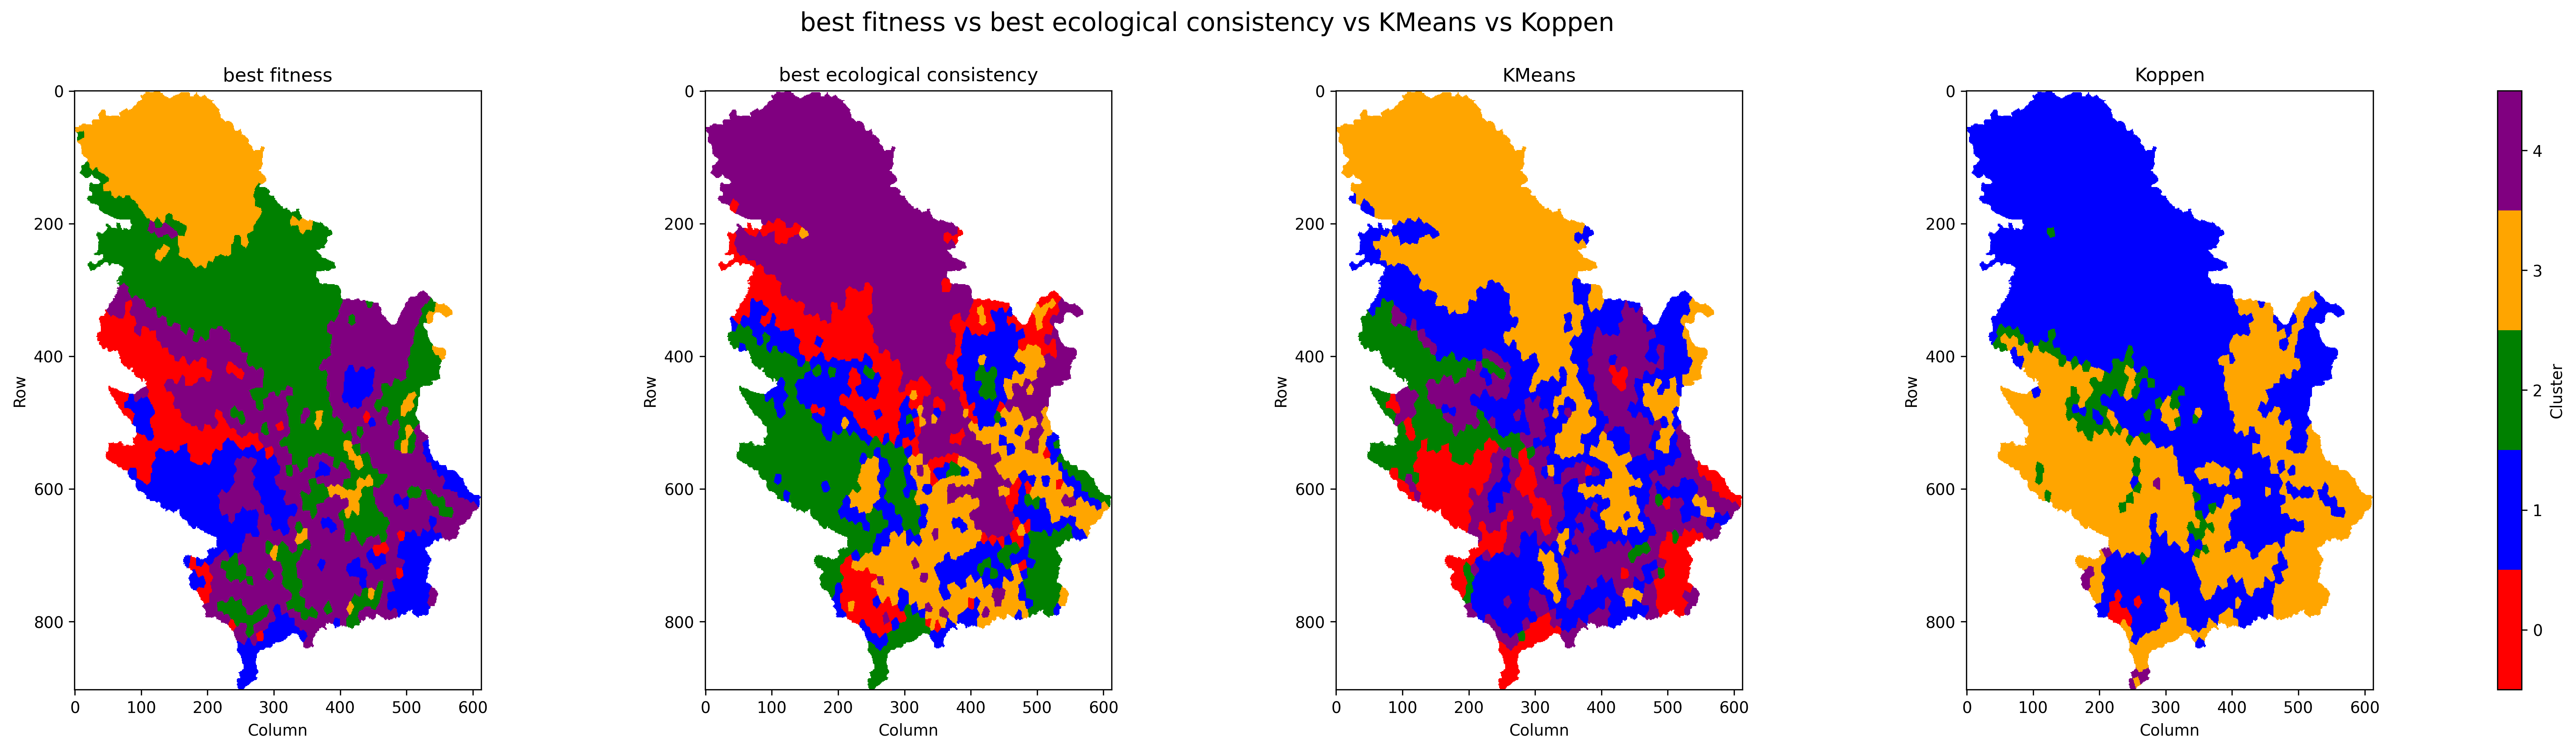
\includegraphics[width=\textwidth]{regionalization_comparison.png}
    \caption{Poređenje najbolje konfiguracije po fitness-u, najbolje konfiguracije po ponderisanoj ekološkoj konzistentnosti, KMeans klasterovanja i Köppen-Geigerove klasifikacije.}
\end{figure}

\section{Dalji rad}
\label{sec:future}

Mogući pravci daljeg rada uključuju ispitivanje drugih reprezentacija klimatskih podataka, razvoj alternativnih funkcija cilja koje nisu toliko vezane za centroide, uključivanje ekološke konzistentnosti direktno u optimizaciju i razvoj feromonskih mehanizama koji su invarijantni na permutacije oznaka klastera. Validacija se može proširiti i na druge nezavisne podatke, kao što su nadmorska visina, tip zemljišta ili dodatni ekološki indikatori.

\section{Zaključak}

Rad pokazuje da je optimizacija kolonijom mrava upotrebljiv okvir za klimatsku regionalizaciju Srbije. Razvijen je kompletan tok rada od klimatskih rastera do regionalizacija, uključujući preprocesiranje, graf susedstva, više ACO strategija, ažuriranje feromona i ekološku validaciju.

Rezultati pokazuju da izbor strategije konstrukcije ima najveći uticaj. Centroidne varijante daju najbolje rezultate, dok graf i kohezioni pristupi u prikazanim eksperimentima postižu slabiji fitness i nižu ekološku konzistentnost. Iako je KMeans veoma jak bazni model za funkciju cilja, najbolja ACO rešenja postižu konkurentne vrednosti i mogu da poboljšaju ekološku konzistentnost u odnosu na referentne regionalizacije. Razvijeni okvir zato predstavlja dobru osnovu za dalja istraživanja klimatske regionalizacije pomoću optimizacionih metoda.

\end{document}
